\section{Instruments}\label{instruments}

Blue instruments are a higher level construct than Csound instruments.
They are designed to allow encapsulating all dependencies together with
the instrument, thus allowing easy sharing of instruments between
projects. Blue instruments may use Csound ORC code,
User-Defined-Opcodes, and f-tables, and they may have a graphical user
interface.

\subsection{Generic Instrument}\label{genericInstrument}

A generic editor for Csound instruments. Insert your instrument text in
the editor, without "instr" or "endin", as they're not necessary and
will be generated by blue.

\subsection{Python Instrument}\label{pythonInstrument}

Use Python code to generate Csound instrument text.

\subsection{Rhino Instrument}\label{rhinoInstrument}

Use JavaScript code to generate a Csound instrument.


\subsection{blueX7}\label{blueX7}

\begin{quote}
\textbf{Note}

This instrument is currently undergoing re-implementation.
\end{quote}

A 6 Operator Phase Modulation instrument using Russell Pinkston's DX7
Emulation Patches.

The blueX7 editor contains two tabs, the 'patch' tab, where the sound
creation parameters are tweaked and a second tab called 'csound' which
can contain further post-processing algorithms or special routing of the
instrument's output.

The patch tab contains three panels: Common, LFO and operators. The
common panel deals with global aspects of the instrument like
transposition, FM algorithm used, feedback, operator enable/disable and
LFO characteristics. The transposition made by Key Transpose is handled
in half-tones, with C3 being the normal (central) pitch.

There are 32 algorithms to choose from which represent the original DX7
possibilities. You can see a visual representation of the algorithm on
the left of this panel.

Feedback represents the amount of feedback into a modulator. The
position and result of this feedback depends entirely on the algorithm
used. The range of feedback is 0 to 7(this range is the same as on the
original DX7). The operator on/off checks turn on and off operators
(current, this is here but the emulation patches do not use them).

The LFO panel sets the global LFO parameters. The parameters are: Speed,
Delay, PMD (Pitch Modulation Depth) and AMD (Amplitude Modulation
Depth). They all have ranges from 0 to 99(the range is the same as on
the original DX7). Additionally you can select the shape of the LFO
from: triangle, saw up, saw down, square, sine and sample-and-hold. You
can also sync the operators: if sync is on, changing Modulation
Sensitivity for pitch (marked with an asterisk *) on any of the
operators will affect the rest.

Finally you have the 6 operators plus an envelope generator (PEG) each
on its own tab. All six operators have the same parameters divided in
the following sections:

\begin{itemize}
\item
  Oscillator
\item
  Keyboard Level Scaling
\item
  Operator
\item
  Modulation sensitivity
\item
  Envelope Generator
\end{itemize}

An important feature of the blueX7 is that it can import DX7 banks. A
large collection can be found in the bigdx7.zip file within the
dx72csound.zip file from:
\href{http://www.parnasse.com/dx72csnd.shtml}{}. (to steven: reading
this page it seems part of the model is unfinished, which may answer
some of my questions above)

On the 'csound' tab you find by default:

\begin{verbatim}
blueMixerOut aout, aout
\end{verbatim}

This routes the output of the instrument directly to the stereo output
of csound. You can include further code to process the 'aout' signal
produced by the blueX7, or to route it as needed. For example, if you
are outputing in mono, you could code such as:

\begin{verbatim}
out aout
\end{verbatim}

To call the blueX7 instrument in the orchestra, create a GenericScore
object in the timeline, and call the the blueX7 instrument. blueX7
requires 2 additional p-fields. P-field 4 is the pitch class of the note
in format octave.semitone (e.g. C4 is 4.00, C\#1 is 1.01 and F6 is
6.05). P-field 5 contains the midi velocity for the note with values
from 0 to 127. For example:

\begin{verbatim}
i1 0 1 8.00 100
i1 + 1 8.02 100
i1 + 1 8.04 100
i1 + 1 8.05 100
i1 + 1 8.07 100
\end{verbatim}

\subsection{BlueSynthBuilder}\label{blueSynthBuilder}

BlueSynthBuilder (BSB) allows the user to graphically build instrument
interfaces for their Csound instruments. The graphical interface is
designed for the use of exploring configuration of an instrument as well
as adjustment to values in realtime(requires enabling using the Csound
API, see \protect\hyperlink{csoundAPI}{here}.

\subsubsection{About BlueSynthBuilder}

It has been my experience that most Csound instruments tend to be
limited in user configurability of parameters than commercial
synthesizer counterparts. It is my belief that a large part of that is
due to the text-based nature of instruments. I've found that:

\begin{itemize}
\item
  Modular instruments are easier to express connections of modules via
  text or code rather than visual paradigms (patch cables, line
  connections), and thus easier to create the instrument by text
\item
  Graphical elements, however, excel in relaying information about the
  configuration of the instrument to the user and also invite
  experimentation, while text-based configuration of instruments is
  often more difficult to quickly understand the parameters settings and
  limits
\end{itemize}

Going completely graphical for the building of instruments, in the case
of systems like Max/PD/jMax or Reaktor, I've found that the instrument's
design no longer become apparent when viewing complicated patches. On
the other hand, using completely textual systems such as Csound or C++
coding, the design of the instrument has a degree of transparency, while
the configuration of the parameters of the instrument becomes difficult
to understand and invites less exploration.

Using systems like MacCsound's widgets or blue's BlueSynthBuilder, one
is able to use graphical elements where they excel, in showing
configuration of an instrument and for manipulation of values, while
using textual elements where they excel, in the design of instruments
and expressing the connections between modules.

I have found that this sort of hybrid design offers the best of both
worlds and when I am spending time building and using new instruments, I
can quickly design an instrument and also explore the parameters of an
instrument's design by using blueSynthBuilder.

\subsubsection{Using BlueSynthBuilder}

BlueSynthBuilder is divided up into three tabs, each of which handles
the different concerns of the instrument builder. Also, the process of
creating instruments and using instruments is also split between
\emph{edit}and \emph{usage} modes. Instrument builders will tend to use
both modes, while users of BSB instruments may not ever have to touch a
line of Csound instrument code or have to modify the instrument UI at
all.

\paragraph{Interface Editor}

The Interface editor has two modes:

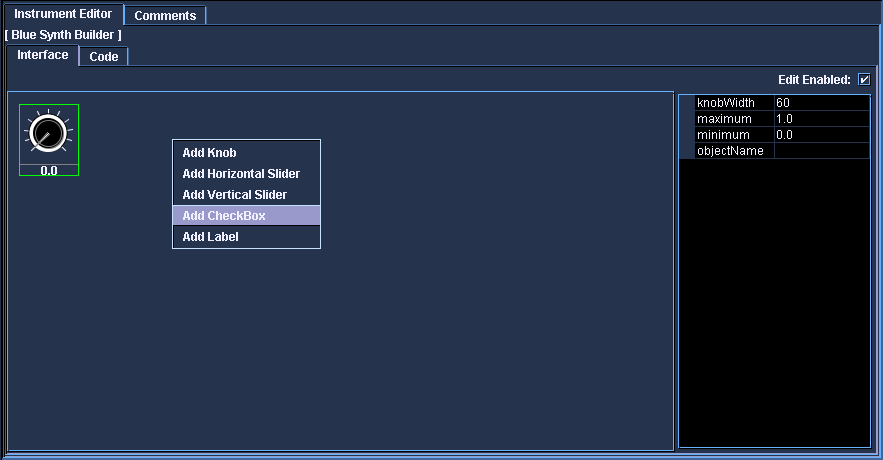
\includegraphics{images/bsb_interface_edit.png}

The user can add interface elements and modify their properties using
the property sheet on the right. To enable edit mode, click on the "Edit
Enabled" checkbox in the upper right of the BSB instrument editor.

Once the edit mode is enabled, right clicking in the main panel will
show a popup menu of available UI widgets for your instrument. After
selecting and inserting a widget, clicking on the widget will hilight it
and show it's properties in the property editor. You can also then drag
the widget around to place as you desire.

You may select multiple widgets by shift-clicking them, or by clicking
on an empty part of the edit panel and dragging a marquee to select a
group of widgets. After selecting multiple widgets, you can drag them
around as a group, as well as use the alignment and distribution options
found on the right side bottom to tidy up the UI.

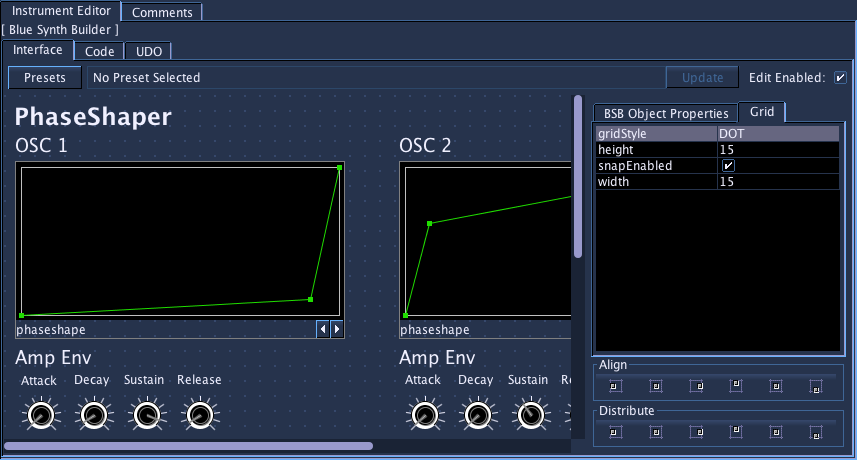
\includegraphics{images/bsb_interface_grid.png}

When in edit mode, you can modify the Grid Settings by using the
properties editor on the right-hand side. This allows you set the
following values:

\begin{longtable}[]{@{}ll@{}}
\caption{Grid Settings}\tabularnewline
\toprule
Property & Description\tabularnewline
\midrule
\endfirsthead
\toprule
Property & Description\tabularnewline
\midrule
\endhead
Grid Style & Affects the visual style of the Grid. Options are NONE,
DOT, or LINE.\tabularnewline
Snap Enabled & Affects whether adding, pasting, and dragging of
BSBObjects in the editor will snap to the grid.\tabularnewline
Width & Sets the width of each grid box. Defaults to 15
pixels.\tabularnewline
Height & Sets the height of each grid box. Defaults to 15
pixels.\tabularnewline
\bottomrule
\end{longtable}

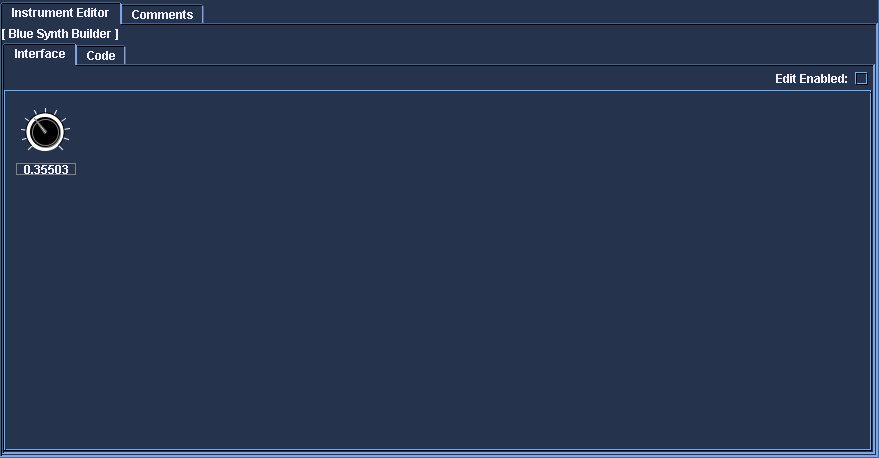
\includegraphics{images/bsb_interface_use.png}

Once in usage mode, users can configure the instrument by working with
the UI widgets: rotating knobs, moving sliders, etc. The values of the
different UI widgets will be reflected in the generated Csound
instrument and will affect the values in realtime if using the Csound
API.

\paragraph{Code Editor}

The code editor is where the Csound instrument code is to be written. To
use the values from the widgets, use the replacement key of the widget
within \textless{} \textgreater{}'s, and that value will be replaced
when the instrument is generated (the replacement key is usually the
objectName of the object; see table below).

For example, if there's a knob with an objectName of \emph{amplitude}
and the value is set to 0.5, the following instrument code:

\begin{verbatim}
iamp    = <amplitude> * 0dbfs
aout    vco2 iamp, 440

        outs aout, aout
\end{verbatim}

will generate the following instrument:

\begin{verbatim}
iamp    = 0.5 * 0dbfs

aout    vco2 iamp, 440

        outs aout, aout
\end{verbatim}

For convenience, the standard code completion popup will auto-complete
text for replacement keys. When editing code, type "\textless{}" then
press ctrl-space. The standard code completion popup will show a list of
all of the replacement keys that have been assigned to interface
objects. Selecting a replacement key will insert that key into the code
text area, already formatted within \textless{} and \textgreater{}.

\subparagraph{Always-On Instrument Code}

MIDI and acoustic instruments often break down into sound generation
qualities that are per-note as well as per-instrument. Having always-on
code that can be encapsulated with the instrument allows modeling things
like body filters as well as adding effects like chorus/echo/reverb to
the instrument itself. While one can always add always-on effects to a
mixer channel, having the capability to add these features to an
instrument can be useful as part of the instrument's design.

To use this, one writes code in teh Always-On code tab. The code from
this tab will be used to generate an instrument that will be run after
the primary instrument code, and will have a single instace of the
generated instrument running for the duration of the instrument. The
signal from the main instrument code should be written out using the
blueMixerOut pseudo-opcode. If the always-on code is disabled, the audio
will go from the instrument to the mixer. If the always-on code is
enabled, the signal generated from the main instrument code will be
intercepted and read by the always-on instrument. To facilitate this
feature, there is blue pseudo-opcode called blueMixerIn:

\begin{verbatim}
asig1 [, asig2...] blueMixerIn        
      
\end{verbatim}

The always-on code should then do processing code, then write out to
blueMixerOut.

To note, BSB widget values work perfectly fine when used within
always-on code.

\paragraph{Widget Values}

The following lists what values the widgets will emit when generating
instruments:

\begin{longtable}[]{@{}lll@{}}
\caption{Widget Values}\tabularnewline
\toprule
Widget & Replacement Key & Value\tabularnewline
\midrule
\endfirsthead
\toprule
Widget & Replacement Key & Value\tabularnewline
\midrule
\endhead
Knob & objectName & float value from knob\tabularnewline
Horizontal Slider & objectName & float value from slider\tabularnewline
Horizontal Slider Bank & objectName\_sliderNum (for each slider) & float
value from slider\tabularnewline
Vertical Slider & objectName & float value from slider\tabularnewline
Vertical Slider Bank & objectName\_sliderNum (for each slider) & float
value from slider\tabularnewline
Label & none & none\tabularnewline
Checkbox & objectName & 1 or 0, depending on if checked or
not\tabularnewline
Dropdown List & objectName & Generates index of selected item when item
is made automatable, or uses value from user-assigned Dropdown
List\tabularnewline
SubChannel Dropdown List & objectName & Value from Dropdown List that is
a named subchannel from the blue Mixer\tabularnewline
XY Controller & objectNameX, objectNameY & X and Y value\tabularnewline
LineObject & objectName\_lineName (for each line) & list of values from
line (can be comma separated, with or without leading 0.0 X value, and x
values can be generated either in absolute or relative
terms)\tabularnewline
Text Field & objectName & Value from text field (compile-time
only).\tabularnewline
File Selector & objectName & If stringChannelEnabled is selected,
outputs a Csound string variable (S-var) that can be updated at runtime
if API is enabled, if stringChannelEnabled is set to off, outputs as a
string (without quotes) at compilation time\tabularnewline
Value & objectName & Generates using its default value or values from
automation. Widget is only visible during edit mode.\tabularnewline
\bottomrule
\end{longtable}

\begin{itemize}
\item
  For the Label object, you are able to style the label by using HTML.
  To use this feature, when setting the text of the label, enter the
  HTML label within \textless{}html\textgreater{} tags, such as
  "\textless{}html\textgreater{}\textless{}font
  size="+1"\textgreater{}My
  Label\textless{}/font\textgreater{}\textless{}/html\textgreater{}".
\end{itemize}

\paragraph{Presets}

Since 0.95.0, BlueSynthBuilder now has the capability to save and load
presets. These presets are for usage-time and not design-time, and they
save a snapshot of all of the values for the widgets. They do not save
x/y coordinates or other configuration for the widget, only the value.

You can add presets and folders of presets using the presets menu in the
upper left of the BSB editor. Each menu has an option for adding a
folder or adding a preset to it. You can also manage presets by using
the "Manage Presets" button. This will open up a dialog with a tree view
of your presets, allowing you to rename the presets and folders, as well
as reorganize by dragging and dropping. You can remove presets and
folders here by right-clicking and selecting the remove option. Changes
in the dialog are not committed until you press the save button, so if
you close the window or cancel, you're old settings will be still in
tact.

\paragraph{Automation}\label{bsbAutomation}

blue supports automation of BSB Widget values for those which support
automation. For these widgets, automation must be enabled before they
allowed to be automated. When making them automatable, the place in
Csound instrument code where the widget value will be added to the
generated Csound code must be a place where a k-rate signal is allowed,
otherwise the code will not compile and Csound will not run the project.
This is required because when using the Csound API, the signal will need
to be k-rate to allow for live modification of the value when rendering.

More information on paramenter automation can be found
\protect\hyperlink{parameterAutomation}{here}.

\begin{quote}
\textbf{Note}

In 0.124.3, a change was made that breaks backwards compatibility.
Previously, if a BSBObject was set to have "Automation Allowed" but was
not itself automated, it would compile as a constant in the generated
CSD. As of 0.124.3, if a widget is made to allow automation, the Csound
code that uses the widget value must accept a k-rate signal, whether the
API is used or not.

If you have a project that rendered fine before 0.124.3 but afterwards
can not render due to problems with Csound complaining that "k-rate
signals not allowed", then you will need to either set the widget to not
allow automation or change the Csound code so that it will work with the
generated k-rate signal.
\end{quote}

\paragraph{Randomization}\label{bsbWidgetRandomization}

Since 0.117.0, users are able to randomize values for widgets in a
BlueSynthBuilder instrument. To use, first choose which widgets are set
to be randomized in edit mode, then in usage mode, right click on the
panel in an area not covered by a widget, then select "Randomize" from
the popup menu. The following widgets are cable of being randomized:

\begin{itemize}
\item
  Knob
\item
  Horizontal Slider
\item
  Vertical Slider
\item
  Horizontal Slider Bank
\item
  Vertical Slider Bank
\item
  XY Controller
\item
  Checkbox
\item
  Dropdown List
\end{itemize}
